\documentclass{article}

\usepackage{graphicx}
\usepackage{tikz}
\usepackage{tikzsymbols}
\usetikzlibrary{calc,patterns,shapes.geometric}
\pagestyle{empty}
\usepackage[margin=0pt]{geometry}
\geometry{papersize={14in,12in}}

\def\centerarc[#1](#2)(#3:#4:#5){\draw[#1] ($(#2)+({#5*cos(#3)},{#5*sin(#3)})$) arc (#3:#4:#5);}

\begin{document}
	\begin{figure}
		\centering
		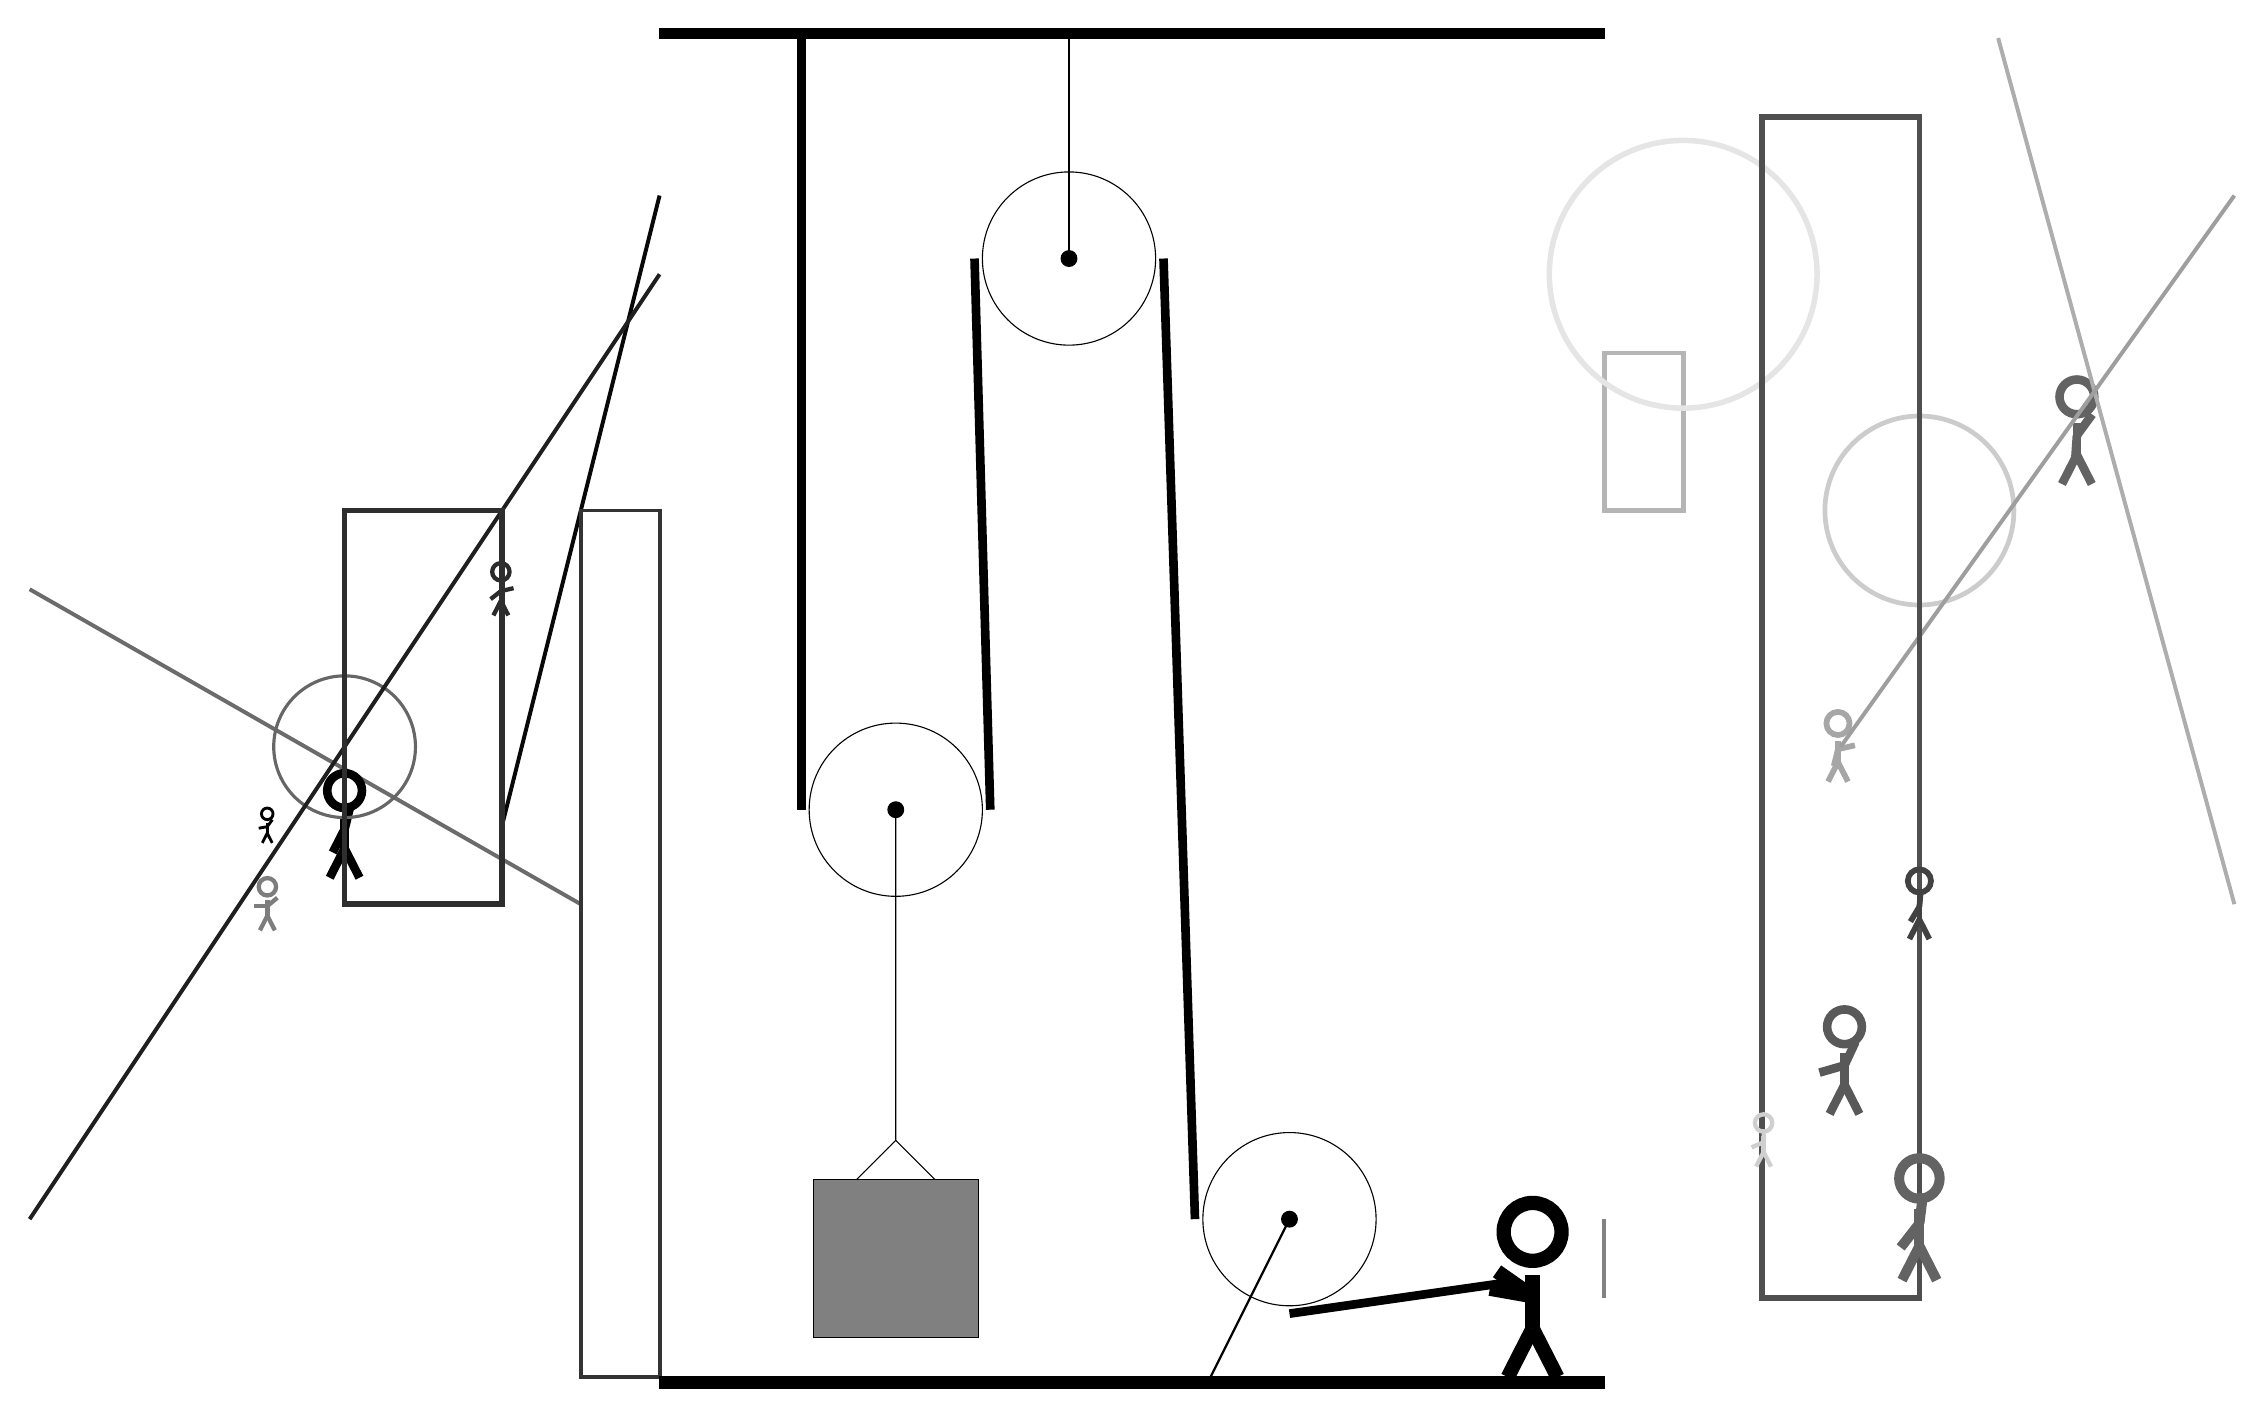
\begin{tikzpicture}
			%%%%% START %%%%%
			
			\draw[fill=black] (-2, 14) rectangle (10, 14.125);
			
			\draw (3.2, 11.2) circle (1.1);
			\draw[fill=black] (3.2, 11.2) circle (0.1);
			\draw[thick] (3.2, 11.2) -- (3.2, 14);
			
			\draw (6, -1) circle (1.1);
			\draw[fill=black] (6, -1) circle (0.1);
			\draw[thick] (6, -1) -- (5, -3);
			
			\draw[line width=0.5mm, color=black!49](10, -1) -- (10, -2);
			
			\draw[line width=0.5mm, color=black!58](-3, 3) -- (-10, 7);
			\node[line width=0.6mm, color=black!100] at (-6, 4) {\Strichmaxerl[6][63][76]};
			\node[line width=0.4mm, color=black!65] at (13, 1) {\Strichmaxerl[6][16][65]};
			\node[line width=0.2mm, color=black!35] at (13, 5) {\Strichmaxerl[4][76][13]};
			\draw[line width=0.5mm, color=black!97](-2, 12) -- (-4, 4);
			
			\draw[line width=0.6mm, color=black!29] (10, 10) rectangle (11, 8);
			
			\node[line width=0.3mm, color=black!61] at (16, 9) {\Strichmaxerl[6][86][54]};
			\draw [line width=0.7mm, color=black!10](11, 11) circle (1.7);
			
			\draw [line width=0.4mm, color=black!60](-6, 5) circle (0.9);
			\draw[line width=0.5mm, color=black!32](15, 14) -- (18, 3);
			\draw [line width=0.6mm, color=black!20](14, 8) circle (1.2);
			\node[line width=0.5mm, color=black!100] at (-7, 4) {\Strichmaxerl[2][10][54]};
			\draw[line width=0.5mm, color=black!88](-2, 11) -- (-10, -1);
			\draw[line width=0.5mm, color=black!38](13, 5) -- (18, 12);
			\node[line width=0.5mm, color=black!83] at (-4, 7) {\Strichmaxerl[3][38][13]};
			\draw[line width=0.5mm, color=black!80] (-3, -3) rectangle (-2, 8);
			\draw[line width=0.7mm, color=black!82] (-4, 3) rectangle (-6, 8);
			\draw[line width=0.7mm, color=black!69] (12, -2) rectangle (14, 13);
			
			\node[line width=0.5mm, color=black!74] at (14, 3) {\Strichmaxerl[4][59][85]};
			\node[line width=0.5mm, color=black!61] at (14, -1) {\Strichmaxerl[7][52][83]};
			
			\node[line width=0.2mm, color=black!19] at (12, 0) {\Strichmaxerl[3][23][89]};
			
			\node[line width=0.6mm, color=black!51] at (-7, 3) {\Strichmaxerl[3][0][40]};
			
			\draw (1, 4.2) circle (1.1);
			\draw[fill=black] (1, 4.2) circle (0.1);
			
			\draw (1, 4.2) -- (1, 0) -- (0.5, -0.5);
			\draw (1, 0) -- (1.5, -0.5);
			\draw[fill=black!50] (-0.05, -0.5) rectangle (2.05, -2.5);
			
			\draw[line width=1.1mm] (-0.2, 14) -- (-0.2, 4.2);
			\centerarc[line width=1.1mm](1, 4.2)(180:360:1.2000000000000002);
			\draw[line width=1.1mm](2.2, 4.2) -- (2.0, 11.2);
			\centerarc[line width=1.1mm](3.2, 11.2)(0:180:1.2000000000000002);
			\draw[line width=1.1mm](4.4, 11.2) -- (4.8, -1);
			\centerarc[line width=1.1mm](6, -1)(180:270:1.2000000000000002);
			\draw[line width=1.1mm](6, -2.2) -- (8.8, -1.8);
			
			\node at (9, -1.9) {\Strichmaxerl[10][-35][170]};
			
			\draw[fill=black] (-2, -3) rectangle (10, -3.15);
			
			%%%%% END %%%%%
		\end{tikzpicture}
	\end{figure}	
\end{document}